%%%%%%%%%%% PREAMBOLO %%%%%%%%%%%%%%
\documentclass[a4paper,11pt]{report}

%%%%% ESTENSIONI %%%%%%
\usepackage[T1]{fontenc}
\usepackage{titling}
\usepackage[utf8x]{inputenc}
\usepackage[italian, english]{babel}
\usepackage{graphicx}
\usepackage{wrapfig}
\usepackage[super]{nth}
\graphicspath{ {./images/} }

\usepackage[nottoc, numbib]{tocbibind}

\usepackage{titlesec}
\usepackage{hyperref}
\hypersetup{
    colorlinks,
    citecolor=black,
    filecolor=black,
    linkcolor=black,
    urlcolor=black
}

\usepackage[T1]{fontenc}

\titleformat{\chapter}[display]
  {\normalfont\bfseries}{}{0pt}{\huge}

\begin{document}
	\begin{titlepage}
		\begin{center}
  			
\includegraphics[height=2in]{Logo_Politecnico_Milano}
  			\vskip.6in
  			\emph{\Huge GAIA\\
			\huge(Get out And InterAct)}
			\vskip.2in
			\Large Design and Technology documentation
			\end{center}

\vskip.6in

\begin{minipage}{.50\textwidth}
  \begin{flushleft}\large
    \textbf{Course}: \\
    \emph{Advanced User Interface}\\
    \textbf {Professor}: \\
    \emph{Franca Garzotto}\\
    \textbf{Academic Year}: \\
    \emph{2016-2017}
    \\~\\~\\
  \end{flushleft}
\end{minipage}
\hskip.1\textwidth
\begin{minipage}{.50\textwidth}
  \begin{flushleft}\large
    \textbf{Group Members}: \\
    \emph{Giovanni Filaferro\\Michele Gennaioli\\Giuseppe Manzi\\Valentina Menabue}\\
    \textbf {Tutors}: \\
    \emph{Prof.ssa Maristella Matera\\Dr. Mirko Gelsomini}
  \end{flushleft}
\end{minipage}

\vskip.4in

\begin{center}
	{\textbf{\Large{Abstract}}}
\end{center}
\par 
GAIA is an interactive toy, which aims to stimulate kids in the first years of primary
school (5/8 years old) to play outdoor and explore natural elements. The device is a tangible band
equipped with 4 bright buttons and 2 speakers tied on a tree. The children interact with the
device through lights, sound and touch. Taking advantages of the
functionalities provided by the device, together with GAIA we designed a possible ideal game to install on it.
The children are driven by an educative story, from a band to another, in a "treasure hunt".
During the entertaining task the children explore the nature and reflect on the moral of the
story.
\end{titlepage}

\chapter{The team}
\begin{wrapfigure}{R}{0.3\textwidth}
    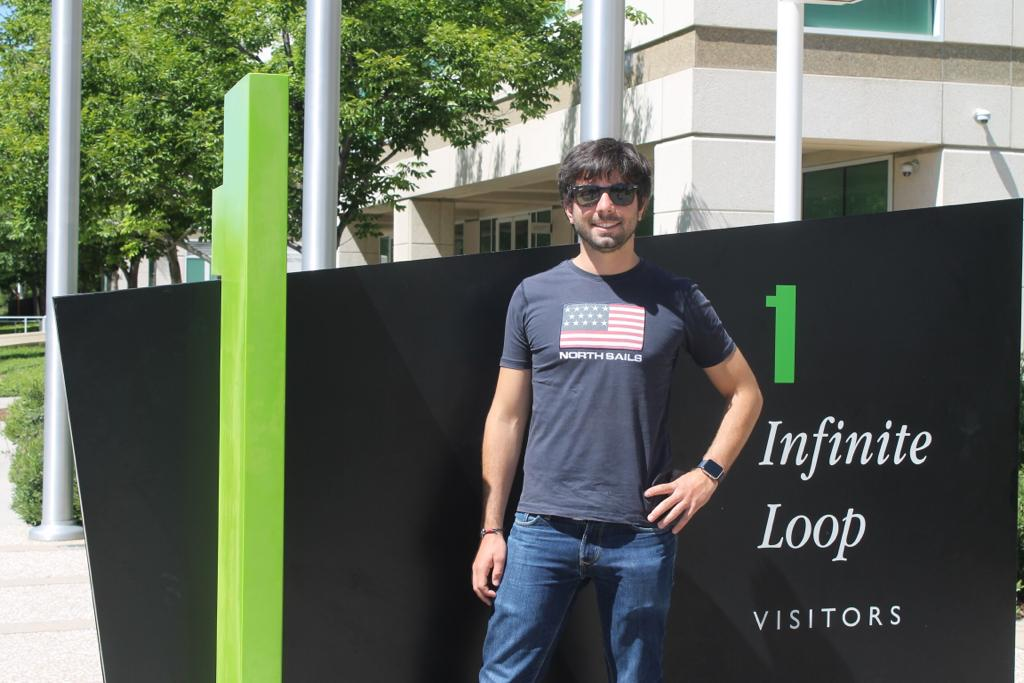
\includegraphics[width=1.2in,height=1in,clip,keepaspectratio]{images/Filaferro.jpeg}
\end{wrapfigure}\par
\\~\\~\par\textbf{Giovanni Filaferro}\par
email: giovanni.filaferro@mail.polimi.it\par
mobile number: 347 4338241
\\~\\~\par
\begin{wrapfigure}{R}{0.3\textwidth} 
    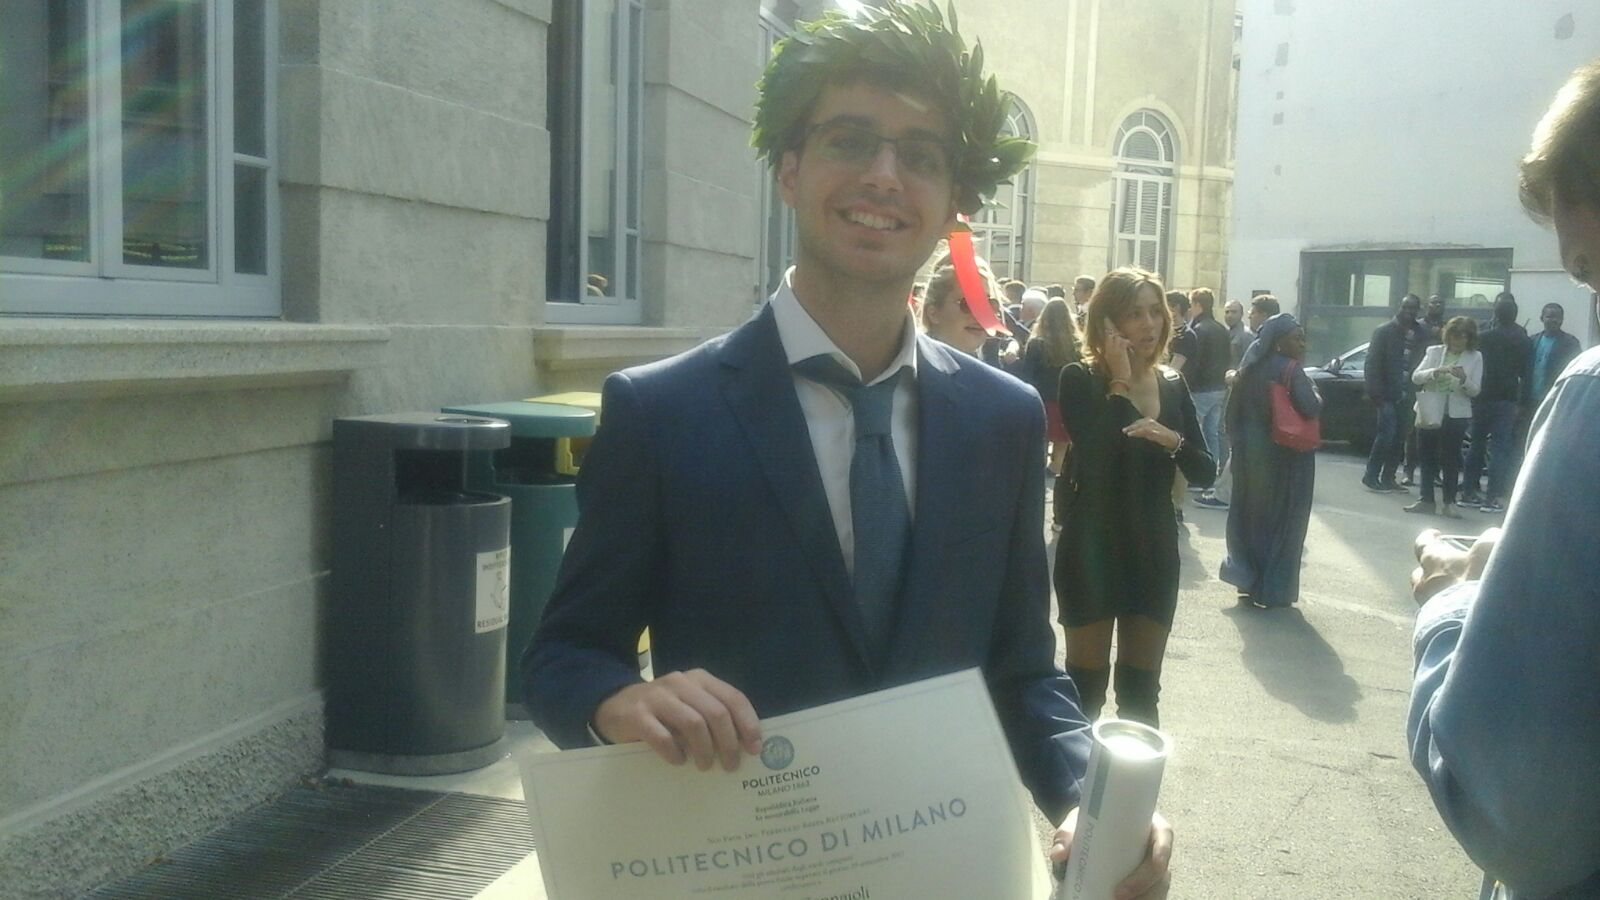
\includegraphics[width=1.2in,height=1.2in,clip,keepaspectratio]{images/Gennaioli.jpeg}
\end{wrapfigure}\par
\\~\par\textbf{Michele Gennaioli}\par
email: michele.gennaioli@mail.polimi.it\par
mobile number: 331 9747877
\\~\\~\\~\par
\begin{wrapfigure}{R}{0.3\textwidth} 
    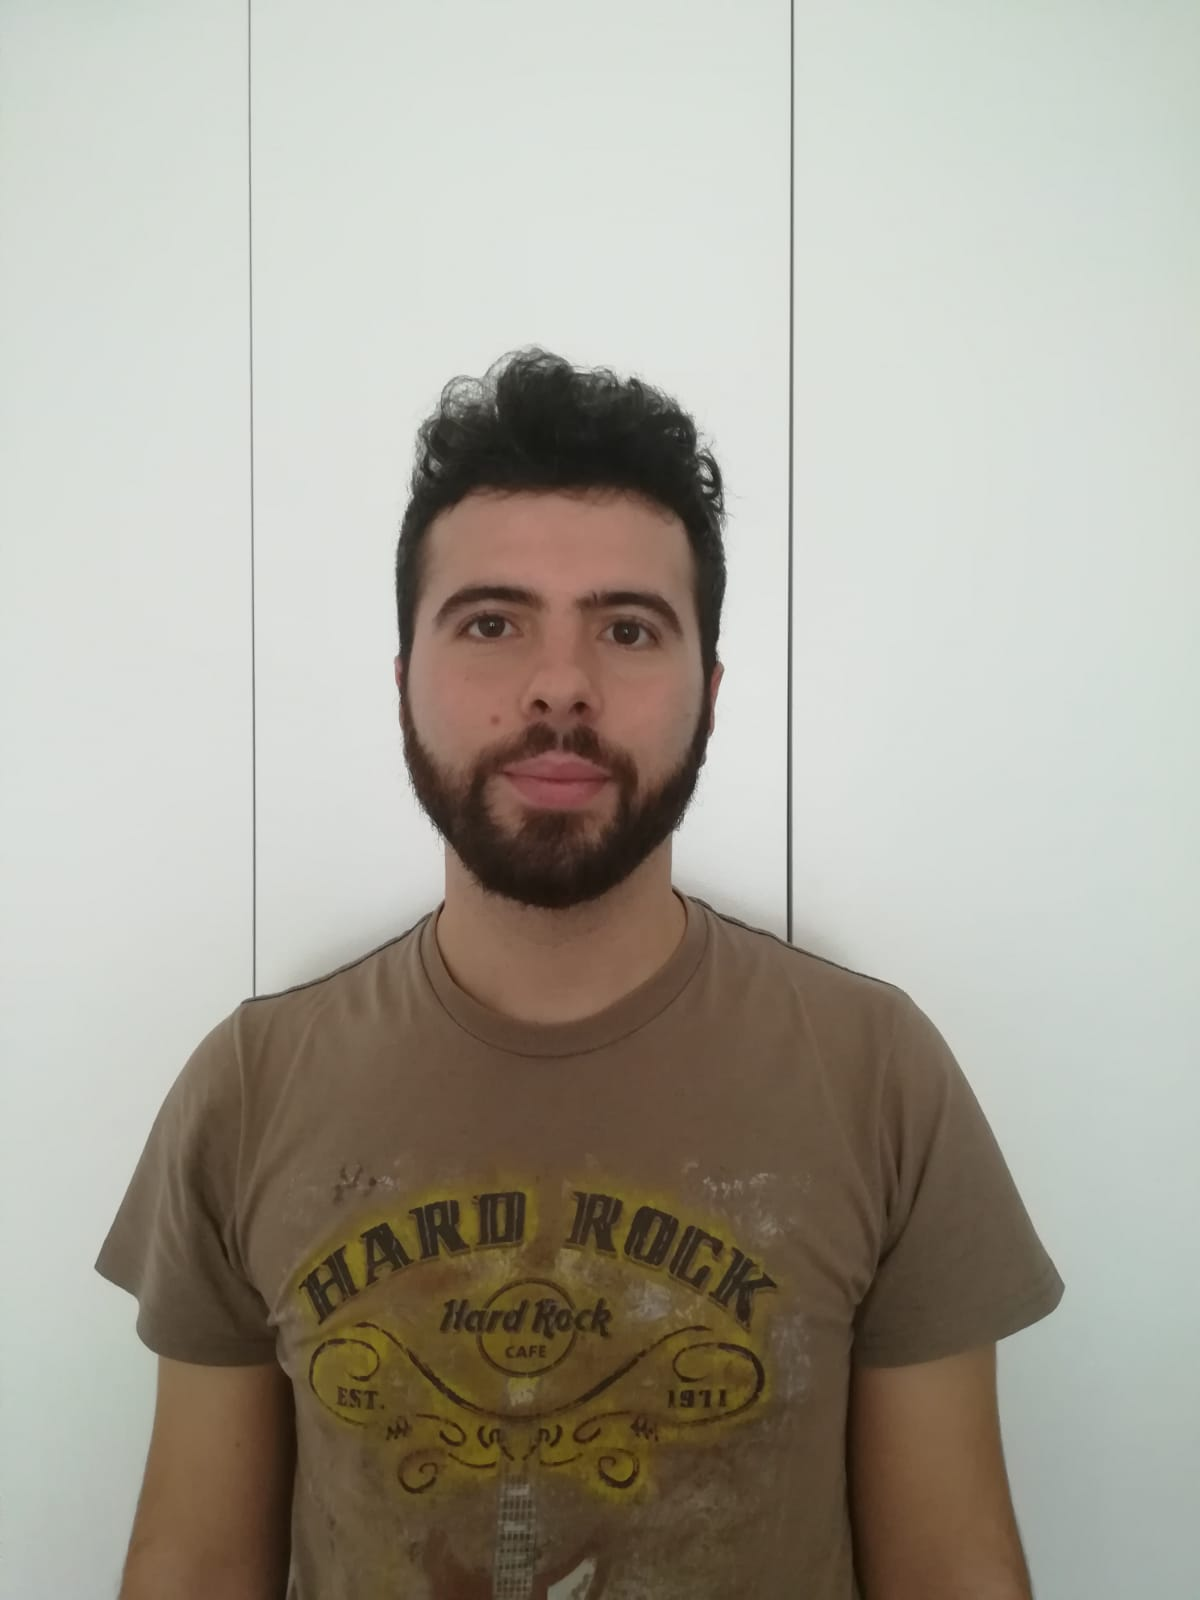
\includegraphics[width=1.2in,height=1.2in,clip,keepaspectratio]{images/Manzi.jpeg}
\end{wrapfigure}\
\par\textbf{Giuseppe Manzi}\par
email: giuseppe1.manzi@mail.polimi.it\par
mobile number: 320 9260703
\\~\\~\par
\begin{wrapfigure}{R}{0.3\textwidth} 
    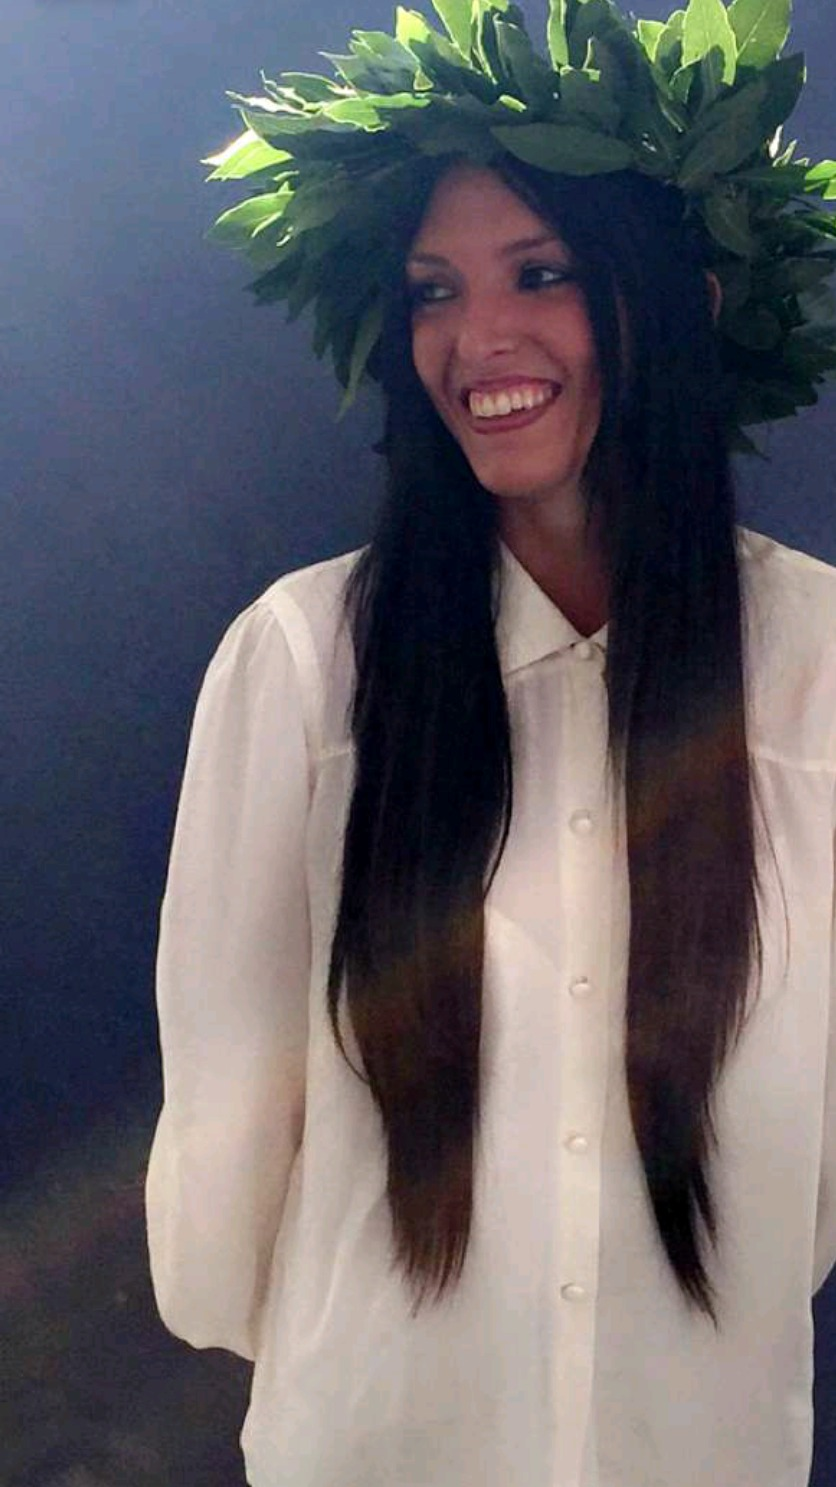
\includegraphics[width=1.2in,height=1.2in,clip,keepaspectratio]{images/Menabue.jpeg}
\end{wrapfigure}\par
\\~\\~\\~\\~\par\textbf{Valentina Menabue}\par
email: valentina.menabue@gmail.com\par
mobile number: 331 2759404
%%%% Inserisce la tavola dei contanuti che va a popolare in fase di compilazione (sono richiesteste almeno due compilazioni, una per generare i riferimenti e una perincluderli) %%%%
\tableofcontents


\chapter{Introduction}
In the last years, the expansion and evolution of smart devices and technology in general has been both an advantage and a disadvantage.
Not only adults, but also children use technology extensively each day. It is a well-known problem that nowadays \textbf{children are more and more exposed to technology}: smartphones, computers, smart TVs, video-games, etc. The attitude of kids to take interest in these systems go hand in hand with the \textbf{trend to play at home instead of spending time outside}. Moreover, smartphones and tablets are becoming a way sometimes abused by parents to entertain children, forgetting that the natural world is a rich and positive resource for the kids' growth and personal development. This has led to the general thought that nature exploration and technology use are contrasting activities. Pervasive games that exploit technology and smart objects have initiated a trend towards solving the tension described above.\par
Starting from these assumptions, confirmed also by some studies, the aim of this project is to \textbf{combine technologies and natural world to encourage children to play outdoors}. We take inspiration from ABBOT, a project developed last year in the same course. ABBOT is a smart toy provided with a camera, which has been developed around four main functions: image capturing, shake and movement sensitivity, colored feedback and data transmission \cite{abbot}. Even though some users involving children showed that ABBOT engages children and motivate them to explore outdoors, on of the identified limits is that each child needs to buy a device, so it appears to become exclusive. Also, Abbot facilitate the exploration by a single child while it did not show appropriate for socialization purposes. To overcome these problems, we developed a device that is supposed to be installed directly outside (in parks), and does not exclude the involvement of groups of children. This allows all kids to play outdoor and socialize with the others, and solves the problem of the exclusivity.\par
As it is well known, the embedded electronics world offers a wide range of usable and adaptable components. This has made possible the realization of a device that includes \textbf{sounds}, \textbf{buttons} and \textbf{lights}. The system is not equipped with a display. This allows to take some distances from the usual digital devices children are used to play with. We thus conceived an interactive system composed of a tangible object (a \textbf{band} to be set on \textbf{trees' trunks}) complemented by a \textbf{game} installed on it: the first one encourages outdoor \textbf{exploration of natural elements}; the second one entertains children. Children's curiosity for the natural world and learning are thus stimulated by combining open-air activities with digital ones, each one amplifying the effectiveness of the other.\par
We named the project \textbf{GAIA}, that is the acronym of Get out And InterAct.\par
This document reports on design, implementation and evaluation of GAIA.
\chapter{Target groups and User needs}
\section{Main Target Groups}
The \emph{main target users} of this project are \textbf{5/8 years old children} (including the one with disabilities), i.e., children of the primary school. Indeed, the first game installed on the device  addresses kids in that age range. However, it is possible to configure any kind of game on GAIA, either simpler or more difficult, in order to make it suitable for other age ranges.\par
The device can also be used in usage situations where \textbf{people with disabilities} are involved. For this reason, the device is totally inclusive.\\
\emph{Secondary users} are:
\begin{itemize}
	\item \textbf{teachers}, that can use the device for structured learning activities;
	\item \textbf{therapists}, that can use the device for interactive activities with patients with disabilities.
\end{itemize}	
Other \emph{stakeholders} are:
\begin{itemize}
	\item \textbf{families}, who cares about their children welfare and education;
	\item \textbf{schools}, that want to exploit new learning methodologies;
	\item \textbf{municipalities} and \textbf{associations}, that can be interested in installing (permanently or temporarily) the device in a park or in any environment where it can support the accomplishment of some learning/education goals.
\end{itemize}
We mainly focused our design on children's and teachers' needs, but we always kept in mind that GAIA had to be adaptable to satisfy the needs of people with disabilities.

\section{Context and Needs addressed}
Some studies assessed that the new digital context offers opportunities for children's learning. However, smartphones and tablets are becoming a\linebreak[4] sometimes-abused way to entertain children, diverting them to the beauty and the benefit of playing in the nature. Starting from these considerations, we decided to design an interactive smart device that exploits new technologies to encourage kids to interact with the nature and learn different important educational values.\par
However, it is not easy to catch the attention of children and make them interested in something. After some considerations and researches, the conclusion we reached was that children can be attracted mostly from lights and sounds, and, at the same time, they need to manipulate something.\par
Our research, in particular, highlighted the following main needs:
\begin{itemize}
	\item Children have the need to \textbf{explore the nature};
	\item Children have the need to \textbf{play outdoors with other children};
	\item Children have the need to \textbf{learn from activities or games};
	\item Teachers have the need to be able to \textbf{customize the game/activity} that they want children to play/do
\end{itemize}
\section{Constraints}
Children are usually indelicate, and they are not aware of how to manipulate digital devices. Having this fundamental assumption in mind, we tried to build a strong and resistant device. In addition the system must be placed outside, so it must be waterproof, lights must be clearly visible, even in sunniest days, and sound must be loud enough to be heard in an open and wide space.\par
Moreover, since the activity should be customized by people with poor or no experience in computer programming or in technology, the device has to be configurable by people that do not have coding capabilities, without relying on external developers.
\section{Goals}
The main goal of the project is to provide the design and a prototype of a \emph{smart device} able to motivate children to \textbf{interact} in many possible ways with the \textbf{nature} while \textbf{enjoying themselves}.\par
However, in order to prove the quality and the potential of the device, it is also important to implement a possible \emph{game} to be played using it, whose goal is to be \textbf{attractive} and \textbf{instructive} and make children \textbf{explore the nature}.
\section{Requirements}
The main requirements are:
\begin{itemize}
    \item	System must be able to react when a disk is pushed
    \item System must be able to play common audio files encoded in common formats (e.g. wav,mp3)
    \item System must be able to light the disks in any RGB colour
    \item System must be able to read a configuration file to execute a sequence of actions
    \item Robustness
    \item Adaptability
    \item Configurability

\end{itemize}
\chapter{State of the art}
Recently, some research communities have been focusing on the domain of nature exploration, and, more specifically, on the problem of \textbf{exploiting mobile technologies to enhance the user interaction with the outdoor environment and the experience of nature}. Most of them are strongly correlated with the use of tablet and smartphones: \emph{LeafSNAP} game proposes a mobile app that identifies plant species through automatic visual recognition and visualizes nearby species localized on a map \cite{leafsnap}; \emph{Geotagger} encourages people to observe the world around them, document what they observe, share it, and foster discussion based on tagged items, bird-watching activity designed using wireless mobile ad-hoc network \cite{geotagger}. These projects, while having the same purpose, differ from GAIA especially for the use of a display, that is an element that can distract the user from the environment around him.\par
However, some projects that don't imply the utilization of an app for smartphones or tablets already exist. They show that, avoiding the use of a display, it is possible to develop games that uses \textbf{technology to stimulate spontaneous social interaction, physical movement and rich face-to-face communication}. This new genre of pervasive games conceived to address this problem is called "\emph{Head Up Games}" (HUGs) to underline that they liberate players from facing down to attend to screen-based interactions \cite{hug}. Some of them are: \emph{Camelot} designed to build a castle with the use of dedicated devices \cite{camelot}, \emph{Stop the Bomb} and \emph{Save the Safe} that stimulate children to revolve around obtaining (or guarding) a key to break into (or protect) a safe using a technological belt \cite{savethesafe}, \emph{HeartBeat} (initially developed as TreasureHunter) that was designed to explore the possibility of using biofeedback in HUGs \cite{heartbeat}. The game we designed for GAIA perfectly fits most of the characteristics of HUGs, since it is an \textbf{outdoor, pervasive game that encourage social interaction and stimulate physical activity, creating a fun experience} \cite{hug}. Moreover, it also has an element that is missing in the aforementioned games, that is the spur to \textbf{explore the nature} that, at the end, leads to an \textbf{educational purpose}. \par
Another playing tool that exploits interaction through sound, light and touch is \emph{Pulse\textregistered}, distributed by \emph{Landscape Structures} \cite{pulse}. It enables some activities like table tennis, tennis, time games. It is a post with a button on its top; it can be set in a park, but it cannot be easily moved. \emph{Pulse\textregistered's} user interface is similar to GAIA's one, but the two devices are very different in the purpose:  \emph{Pulse\textregistered's} only aim is to make children \textbf{enjoy themselves in the outside}, while GAIA is also thought to make children \textbf{get in touch with the nature}, so it can be set on a natural element, and it allows children to explore a different point of the park just moving the band to a different tree. 
\chapter{Solution - UX Design}
\section{General approach to address the problem}
GAIA experience is based on the use of a tangible smart device that uses sensors and actuators to attract children outdoors. The aim of the object is to interact with children making them explore the nature and to provide educative content. For this reason, during the interaction, the children hear a story that drive them around the park.
\section{Details of interaction and interfaces}
GAIA allows kids to hear sound, see lights and interact through touch while they are enjoying the natural world. The smart object is a \textbf{band with LEDs, speakers and buttons managed by a microcontroller}. Four LEDs and push-buttons are set on a \textbf{3D-printed semi-transparent white disk}, that diffuse the light. Each band is equipped with \textbf{4 disks that can emit light and react to the pushing}. Two speakers on the band allow the \textbf{playing of sound}. It is possible, in this way, to have a \textbf{wide number of possible flow of interactions}. All these features make the device appropriate to many kinds of activities both outdoor and indoor.  Indeed, the main idea is to use it to encourage children to play outside, but it can be used also for many educative activities inside schools, houses or institutions for people with disabilities.\par
Among all the possible interaction flows that GAIA is able to provide, one that is very interesting and shows all the potentialities of the device, is the game that we provide together with the device. By getting inspired from one of the most popular traditional activity that enables wide area exploration, that is treasure hunt, we designed a game that uses \textbf{a set of GAIA devices} (for our prototype we used 3 of them) \textbf{as checkpoints in a path around the park}.\par
Each band is set on a tree spread in the park and tells the chapter of a story. The first tree is the only one having bright disks and, when any button is pressed, it starts reproducing the first chapter of the story. At the end of the telling, the system lights a disk and a user is asked to remember the colour he/she sees. As soon as the user memorizes the colour and pushes the button, GAIA reproduce the audio file containing the description of the next tree. When the user has reached the next checkpoint, he/she has to insert the colour that has been showed at the previous step, and then the interaction follows as described for the first tree. This procedure goes on until the story terminates. When the children reach the end, they explored the park and, in addition, they learned the educative moral of an attractive story.\par
Many of the elements of a traditional treasure hunt are present. Besides \textbf{the presence of a path having checkpoints}, we can identify:
\begin{itemize}
	\item \textbf{A reason to search the next checkpoint}, that in the traditional game is due to the willing to find a treasure, while in the GAIA version is obtained thanks to the suspense created at the end of each chapter.
	\item \textbf{The hint that enable the research of the next checkpoint}, that in the GAIA version is the description of the tree
	\item \textbf{The password to give access to the checkpoint’s information} (in some traditional treasure hunts some clues has to be decrypted using the key given at the previous step in order to avoid the skipping of some part of the path), in the GAIA version is the colour showed 
\end{itemize}
All the actions the user has to do to complete the hunt are explained by audio instruction. Key points for the good success of the game are the \textbf{quality of the story} and the \textbf{clarity of the descriptions}. For these reasons, we involved some \textbf{teachers in the review of the story}, that is an original one we had written, \textbf{and in the writing of the descriptions of the trees}. Moreover, it is essential to have a \textbf{good interpretation of the story that keeps the attention of the children high and captivates them} enough to stimulate the willing to go on in the hunt. For this reason, we asked to a professional actor to record the audio files.
\section{Relevant Scenarios}
We mainly focused our design on children’s and teachers’ needs, so we provide the two scenarios related to these type of users, even if GAIA can be useful also in a therapeutic environment allowing people with disabilities to make some activities.
\subsection{One child in a public park}
Mary is a 5 years-old girl. She likes playing outdoor, but their parents are always too busy so, she usually has to stay at home. Mark, Mary's father, heard about an interactive treasure hunt organized in "Parco Lambro" by an association. This Sunday he has no commitment, so he decides to bring Mary at the park.\par 
As soon as they arrive, a guy explains that Mary simply has to find and get close to a speaking tree, and from there a treasure hunt will start. While exploring the park, she sees some lights coming from a tree. Mary is very curious, so she gets close to the tree. A voice is coming from the tree and asks her to touch a button if she wants to play. The girl presses a green button. Mary quietly listen to the beginning of a story. Unexpectedly the story stops in the thick of it. Mary really wants to know the rest of the story. GAIA shows Mary a blue disk and asks her to remember its colour. Then the band describes a tree and explains to Mary that she can hear the rest of the story only if she finds and reaches it.\par
Mary, accompanied by her father, goes around the park to find the next tree guided by the clues previously listened. She finds the tree. Mary is very happy to see that another band is set on the tree, so she immediately pushes a button. GAIA asks her to hit the disk having the colour she previously memorized. Mary has good memory skills and touches the blue button. The tree starts to tell the next chapter of the story. At the end, the bend lights a yellow disk and Mary memorizes it. Then another tree is described. This allows the girl to find the next tree and continue the story.\par
The child goes around the park to find the next tree guided by the clues previously listened. She finds the tree. Mary hits a button and, when asked, touches the yellow disk. The tree starts to tell the final chapter of the story.\par
Mary and Mark go back to the entering of the park. Here the same guy who welcomed them when they arrived asks Mary what she has learned from the story. The girl, who listened carefully to the telling, answered: "We have to respect the nature". The guy tells Mary he is very proud of her and she deserves a prize, so he gives her a small stuffed squirrel, the mascot of the story.
\subsection{A group of children in a school yard}
Kate is a science teacher in primary school. She just finished a set of lessons on the characteristics of trees, such as leaf shape and bark colour, so she wants to test her 7 years-old students on what they learned. She likes innovative teaching, so she decides to use GAIA, a new technological device, to check her students' knowledge while they're enjoying themselves. She records some descriptions of the trees present in the school yard and uploads them on the device. Then she divides the class in groups of 4 children and take one group at a time from the classroom.\par 
The first group is led to the starting tree. The tree is speaking, they all are very curious. The tree asks the children to touch a button if they want to play. The children press green button. The tree tells the beginning of a story. At the end the tree. The tree asks to the children to press red button and remember that colour in the future. Then the first description recorded by Kate is played. Children discuss about which could be the right tree, and Kate takes notes about how much they learned during her previous lessons. When all the group agrees on the next tree, they reach it. Kate notes that they found the right one. \par 
As they did for the first tree, the children push a button to let the play start. GAIA asks which was the colour they memorized, but Paul, one of the members of the group presses the green disk. The band plays an error message and asks to insert the colour again. Paul's mates explain him that the colour was red. They press the right disk all together. GAIA starts to tell the next chapter of the story. At the end, the tree asks to them to press yellow button and remember that colour in the future. Then the tree plays the second description recorded by the teacher.\par
Kids go around the park to find the next tree guided by the clues previously listened. They find the tree. The band asks for the colour they previously memorized. This time they talk before hitting a button, and, thanks to cooperation, they don't make any mistake. The tree starts to tell the final chapter of the story.\par
The group is happy to have heard a nice story and they all get a good mark since they managed to find the trees and cooperate to be successful.
\chapter{Solution - Implementation}
\section{HW architecture}
The device is a band having 4 disks (we call them DOTs) and 2 speakers. Each DOT is 3D-printed using white PLA filament and contains 4 RGB LEDs and 4 push buttons in parallel.\par
All the electronics concerning the single DOT is made of a custom PCB (which could support up to 7 DOTs connected in series).\par
The components are controlled by a single-board computer (Raspberry Pi Zero W) and powered by a 10000mAh power bank.\par
This microcontroller is supported by a custom hat PCB which features:
\begin{itemize}
    \item Power Supply distribution
    \item Audio filter and its relative amplifier
    \item Pull down resistors for buttons
    \item Voltage divider for LED signals
    \item NFC pins for future implementation
    \item Exit connector for the DOTs and speakers as well as for the 2 proximity sensors inputs (for future implementation)
\end{itemize}
This structure and the battery are both placed in a custom 3D printed case.\par
The whole band, except for the disks’ surfaces, is made of Neoprene fabric. The neoprene used for the prototype isn’t waterproof, however many waterproof versions are available on the market.\par
The whole band has some rivets (at the beginning and in the end); this enables flexibility for the band to be placed in different trees whit different trunk sizes.

\section{SW architecture}
The Software is built as a customized service for the raspberry pi operative system (Raspbian).
It is completely built in python (version 3.7) and can be easily uploaded to a new board just by using some pre-built bash scripts via SSH.
Our implementation is completely customizable, just by editing a custom file type based on JSON syntax. 
There are pre-defined sets of actions that combined together can create an unlimited variety of games. This actions can be further extended creating custom ones (which inherit from the base action class) and then can be used in the action file to create new interactions.
The one that we have implemented are:
\begin{itemize}
    \item Restart Action (restarts to the original state of the game)
    \item Play Audio Action (plays an audio file)
    \item Show Color Action (shows a color in the specified DOTs)
    \item Play Animation Action (plays pre-defined animation on the DOTs)
    \item Dynamic Load Action (loads an action file and appends them at the end)
    \item Jump Action (jumps to a specified action)
    \item Wait Input Action (waits a specified input before starting the next action)
    \item Delay Action (waits a delay)
    \item Combined Action (executes in parallel some specified actions)
    \item Single Selection Menu Action (defines a menu of choices)
    \item Multiple Choice Menu Action (defines a menu with multiple choices) 
\end{itemize}

\chapter{Empirical Evaluation}
To evaluate the user experience and the design of GAIA we led 4 studies. Two of them were interviews with teachers, two were user studies with children.
\section{Teachers interviews}
\subsection{Research questions and variables}
The interviews with teachers aim to understand \textbf{the weaknesses and the potentialities of GAIA}.\\
The main information we wanted to get from the teachers were:
\begin{itemize}
	\item if they \textbf{identify in the technology a possible solution} to the problem of the decreasing time children spend outdoor;
	\item if they have ideas about \textbf{how to use technology to stimulate nature exploration};
	\item if they have ideas on \textbf{how to use GAIA};
	\item if they have suggestions about \textbf{the game we designed}.
\end {itemize}
\subsection{Participant profile and context}
We led \textbf{two different interviews}. The first one was held on the \nth{19} of December. We interviewed \textbf{4 kindergarten teachers}. Three of them were aged between 46 and 60 years old, one was aged between 31 and 45. Only one of them feels uncomfortable in using new technologies. They all frequently use smartphones and computers in everyday life, half of the interviewed teachers also use tablets. During their teaching activities, only 2 of them are used to ad hoc technologies, such as computer and IWB (that is also occasionally used by another of them). None of them is familiar with the term "smart toy".\par
The second study was held on the \nth{21} of January. \textbf{Seven primary school teachers were interviewed}. Among them, 3 were aged between 46 and 60, 2 were aged between 31 and 45, and 2 were less than 30 years old. All of them feel quite comfortable in using new technologies, one in particular feels very confident.  All of them uses computers and smartphones in their everyday life. Just one doesn't use the tablet. Two also have a smart TV. During their teaching activity, 3 of the interviewees use IWB. Two of the interviewed teachers have an idea of what a smart toy is.
\subsection{Data gathering} 
Each interview was divided in \textbf{two phases}. During the first one teachers were asked to \textbf{fill in a questionnaire} about their profile, their opinions on children outdoor playing and their ideas about the opportunity to use interactive attractions to stimulate outdoor playing.\par
The second phase was structured as a \textbf{focus group}, during which they discussed together their answers to the questionnaire, the ideas about possible uses of GAIA and their considerations about the game we designed.
\subsection{Execution}
After a short presentation, the teachers were asked to fill in the questionnaire on their smartphones and, then, to freely discuss aloud about their thoughts regarding outdoor playing and technology. During this phase they didn't know anything about the project we are leading, so that their answer were not influenced by our work. For the same reason, before asking ideas on how to use GAIA, the device was shown and presented, but nothing was explained about the game we designed. Finally, after a short game demo, the teachers were asked to provide some advises about the interaction flow and the contents of the game.
\subsection{Results and discussion}
The main worry that emerged from the interviews was that GAIA provides light and sound stimuli, to which nowadays a child is already too much exposed. For this reason they identify the device as a \textbf{support for "structured activities"}, and not as an object to be set permanently in the park. In such a way the \textbf{stimuli are provided only when needed} and the children can normally explore nature without been distracted by lights. \textbf{They proposed some interesting activities that can be done thanks to the support of GAIA}, such as "Strega comanda colore" (a popular Italian traditional children game, during which a child orders to their mates to touch a specific colour and that is used by kindergarten to teach colours), tests on left and right directions, tests on cardinal points, classification tasks, "\textbf{routes with lights and voice}", "\textbf{a treasure hunt}" (specifying that they had to think on how to set it up). In particular, this last two proposals, that arose spontaneously, are consistent with our idea of game. \par
The teachers were also asked to express their opinion on the game. All of them \textbf{embrace positively the game idea}. Also the ones that had previously express doubts about the use of technology to explore the natural world, changed their minds ("if used in this way, technology can be a nice solution"). They were worried about the presence of two different games since we showed them a version of the interaction flow slightly different from the actual one. The user had to remember a sequence of colours instead of a single one. This could be, in their opinion a problem, because it could distract the children from the story and from the tree descriptions. This is the reason why the actual version uses a single colour. \textbf{Teachers were also asked to review the story that had been written}. They approved most of plot and appreciated the interpretation of the actor that recorded it. They asked to change some elements in order to eliminate an inappropriate behaviours of the main character, to have a different ending and to insert more natural elements, avoiding a mix between nature and fantasy.
\section{User studies with children}
\subsection{Research questions and variables} 
To get the best results from the user study, we first designed and planned it, trying to focus on testable variables. The first step was to identify the topics of interest then we refined the general idea into a precise question to be studied by gathering and analyzing data. To be more accurate we divided the metrics into two parts.\\
Quantitative metrics:
\begin{itemize}
	\item Number of children that have difficulties or don't get close to the device.
	\item Number of failed touches
	\item Mean time of discussion between children to identify the next tree
	\item Mean time for a tree
	\item Mean time to reach the next tree
	\item Mean time to conclude the game
\end{itemize}
Qualitative metrics:
\begin{itemize}
	\item Difficulty to play (perceived from observers)
	\item Difficulty in the use of the device (perceived from observers)
	\item Ease distraction during the game
	\item Unplanned behaviours 
	\item Unplanned use
	\item Difficulty to play (perceived from children)
	\item Difficulty in the use of the device (perceived from children)
\end{itemize}
Moreover we made a questionnaire to analyze children's satisfaction to be completed at the end of the game. In addition, we prepared some other question for \textbf{interviews with some children}. During the study we had the possibility to \textbf{make some videos to record the reaction of children}. At the end of the experience we gave to children, as an incentive, a participation certificate. 
\subsection{Participant profile}
We had the possibility to conduct \textbf{two studies} with children of different ages, different schools and different classes.\par
The first one involved \textbf{23 five years-old children of a kindergarten}. Teachers helped us dividing them into 4 groups (one of three children, one of four, one of six, one of ten).  The second one involved \textbf{49 children of 7-8 years old attending the second and the third years elementary school}.\par
The configuration of the device and the one of the game were identical for both the studies. The only differences were the description of the trees and their relative distances. For younger children we recorded simpler descriptions with easy-to-spot characteristics (size of the tree, nearby park facilities, etc.) and we chose trees that are close to each other. For 7-8 years-old children we recorded descriptions containing technical details (shape of the leaves, exact name of the plant, etc.) and we choose trees that are quite distant from each other.\par
The choice of the trees was discussed with the teachers of the two schools, as well as the technical description for primary school children were readapted starting from the ones they wrote for a herbal.
\subsection{Context}
The 24th of January we started at 9:00 with the children attending the kindergarten in Via Gallina, Bareggio (MI). The park of the school was fine but not so big. It was equipped with some park facilities such as a red little house and a slide that we inserted in the description to ease the task of the children. The study at kindergarten finished at around 12:00 p.m. At 1.00 p.m. we started to Via Sturzo in Cornaredo (MI) the study with elementary school's children. The park of the school was very big. The study lasted until 4.00 p.m. 
\subsection{Data gathering} 
Data collection involved structured observation based on \textbf{video recordings to analyze playing behaviour}, and \textbf{questionnaire-based interviews}. The adopted measurement instrument for the questionnaire is an iconic form that allows children to express their preferences. To answer the first 4 questions the children had to use a "\textbf{smiley-o-meter}" based on a 5-point Likert scale \cite{smileyometer}, while the last two answers were multiple choice questions, with 3 possible answers (yes/no/maybe). We took into account the kids? ability in reading and comprehending textual content. Since the children of the kindergarten were not able to read, we drove them in the compilation. Knowing that usually children try to copy each other, we tried as much as possible to make them complete the questionnaires individually. 
In addition, \textbf{we interviewed some children and took notes about their opinions}. 
The video we were able to make are very useful to make a deeper analysis of time variables and reaction of children. 
\subsection{Execution}
We conducted an exploratory study to assess kids' attitude towards the playing experience using GAIA, to verify whether \textbf{different ways of approaching the device and the game exist according to the kids' age}, to get \textbf{further indications on the usability of the physical object}, and to \textbf{understand if the game can stimulate to move around the park without difficulties}. Kids' parents were asked to sign an informed consent, including explicit agreement for each child to appear in video recordings and to use the collected data in our research. The study was organized into four phases: \textbf{introduction}, \textbf{play}, \textbf{administration of questionnaires} and \textbf{interviews}. The school teachers also attended the study sessions and helped us, when needed, in the explanations given to children during the introductory phases and in controlling the groups during the game play.\par
The first phase was held indoor, in one of the school classrooms. One of us gave a 5-minute introduction, to introduce ourselves and ask children if they like play outdoors. As we expected, almost all of them gave with much enthusiasm a positive answer.\par 
After the introduction, each group of kids was asked in turn to go outdoors, in the school garden. The aim was to observe if children were attracted from the device and if they want to move close to the band. \textbf{The children's attention was immediately captured by the bend}. Every group asked the teachers the permission to get nearer and they easily understood they had to push a disk to activate the device. The audio output of the device was lower than expected, since it has to propagate in a big open space. However, this led the children to \textbf{stay quiet and lean their ears on the device to hear the recorded voice}. After hearing the end of the chapter most of the children immediately run toward the next tree, without hearing the description, but just attracted by the view of another band. This behaviour was in some cases \textbf{corrected by other members of the group}, in other cases by the teachers or by the conductors of the study. Children always made more hits on the buttons than the ones strictly necessary to complete the games. This was either due to the enthusiasm in exploring the device or to the presence of several children around the band. In the second case, some groups were able to \textbf{discuss and regulate the behaviour in order not to touch the wrong colour} when an input was requested.\par 
After they reached the end of the game, the children were led back to the classroom, where they were asked to fill out a questionnaire. During this phase some of us had the possibility to ask some question to children in order to understand if they liked the experience, if they had some problems interacting with the device, if they would like to change something, if they had suggestion on other games to install on GAIA. While a group were involved in the game, one of us took care of the other children that remained in class, asking them to \textbf{fill out the questionnaire} and perform alternative activities that provided us with additional useful material to take ideas on how to improve the system. We made them draw a three with some games they desired on it. Some interesting ideas came out, in particular, we noticed that most of them, in their drawings, make a \textbf{correlation between nature and video-games}.

\subsection{Results and discussion}
Through the questionnaire we were able to get some numerical values. We used a \textbf{spreadsheet to collect data}. For each child we identified: code, gender, age, school, group and finally the six questions Q1, Q2, Q3, Q4, Q5, Q6. Each field has a range of value. The code is an increasing number. The gender is 1 for female and 2 for male. The age is the number equivalent to the age of child. The school is E if the child belongs to the elementary school and M if the child belongs to the kindergarten. The group is an increasing number. The domain of first four questions goes from 1 (at all) to 5 (very much), while the domain of questions 5 and 6 is \{0(no), 1(maybe), 2 (yes)\}.\par
Inserting values in this table we got some statistical results: the median, the mean and the variance. Unfortunately, these data are not very reliable: it is known that children use to sign the smiley they like most and they are influenced by others and by the game situation.\par 
It was important to notice the reaction of children in front of the device. \textbf{They were fascinated by the lights} ("They look like a rainbow!") \textbf{and by the sound} ("This thing is talking! What is this strange stuff?"). Since the volume was low, they had to stay quiet and whenever somebody talked while the story was playing, their mates scolded him/her. This was clear evidence of the \textbf{involvement they had in the story}. The fact children often run toward the next tree without hearing the description is both a symptom of a non-perfect clarity of the game instruction and, at the same time, a sign of the \textbf{eagerness to go on in the exploration}, that is a positive result.\par
As suggested by the teachers during the interviews, we observed that children of all ages have an \textbf{excellent experience if they’re supervised during the game}. We avoided non-supervised game experiences, since the teachers had to stay close to the students for legal responsibility reasons and the children were aware of this condition, in fact they always asked permission before walking away.\par
Other interesting behaviours are observed whenever a member of the group has some limitation in what he/she can do during the game. Two groups, in particular, experienced a situation of this kind. A group included \textbf{a member affected by Down syndrome}. He was perfectly integrated by his mates and \textbf{had no problems in using the device}. Another group included a member who had health problems during the past two weeks and so he was asked not to sweat. All the group perfectly understood the situation autonomously and moved from one tree to the next one without running.\par
The most interesting fact we observed was the \textbf{willing to continue exploring the nature}, even after the end of the game, originated by the GAIA experience. The primary school park hosts some squirrel. Some of the kids were able to look at the foliage of the last tree and identify one of them in the leaves (“This story is real!”). Others saw a squirrel climbing on a trunk just before re-entering in the school. Most of the children were happy to loudly call “Polly” (the name of the mascot of the story), hoping it will show up to them.\par 
\textbf{The majority of the kids liked the story}, someone asked to continue it. The older kids also understood the moral of the story and some of them kept reflecting on that with the interviewers after the game.\par
Due to the need of continuous maintenance of the device during the study and lack of time, it was possible to note in real time the data for quantitative measures, so our future work is to extract values from the videos we took.
\chapter{Value Proposition}
This document has presented the design of the GAIA interactive game as a mean to encourage kids to explore nature. Thanks to the proper use of technology, through GAIA, open-air activities also become an opportunity to acquire knowledge in the context of a smart and educational setting.  We believe that our device has a great potential: \textbf{GAIA can support a huge range of activities and it is adaptable for a great variety of users and environments}. Since we wanted to build a multipurpose object addressed to children, we met some hurdles. Indeed, at first we needed to empathize with children to understand their tastes. The choice of which game to install on GAIA was hard because our goal was to combine fun with learning. To solve this problem we decided to interview teachers, since they work everyday with kids. They gave us some useful advices on the game, and in general, on the activity to install on GAIA. Another important challenge for us was building the device from scratch. Assemble all pieces and make them resistant to touches took us a lot of time. \par
We included in the project the most versatile and user-friendly interaction enabled by a smart object, those that could attract more a child: the touch, the view and the listening. This has led to a \textbf{really adaptable device}, that has been designed to be permanently set in a park, but has features that make it useful as a \textbf{support in many other outdoors and indoor activities}. That’s the reason why \textbf{the greatest feature of GAIA is its adaptability}.\par
It is possible to find some similar devices and competitors on the market, but our original product differs from others not only for the shape but also for the contents. Indeed, \textbf{there are no similar objects that correlate playing activities with educative ones and that, in addition, encourage people to play outdoors}. Moreover it is difficult to find \textbf{such an high degree of flexibility to different contexts} in other solutions available on the market.
\chapter{Future work}
GAIA is still in a prototype version. So far our work has especially concentrated on designing the interactive service and on analyzing its acceptability by kids and its feasibility by means of state-of-art technologies and the interviews with the teachers. Some refinements have to be applied to exploit all its functionalities. From a structural point of view, since it is a device supposed to be used outside, GAIA must become waterproof and more resistant to weather events. At the same time, substituting the normal buttons with capacitive fabric would be a good idea to exploit the whole surface of the band. From the implementation point of view, the configuration file and the algorithm can be improved. In this first prototype we didn’t want to stress and test extensively this aspect, as we were more interested in evaluating the validity of the overall concept as a tool for outdoor exploration and learning. Improving the configurability enables the implementation and the installation on the device of different kind of games or activities.
It is possible to improve the game of the “treasure hunt” using RFID cards representing characters, settings, or other elements of the story. These kind of instruments make possible the recognition of a story, thus the possibility to have different types of stories. In addition, children would be happy to collect and exchange them.
Another issue to take into consideration is that the devices (the trees) are not linked. It is planned to connect them through wireless mesh WiFi. 
Moreover to stimulate more the users during the play it can be possible to make an interaction between GAIA and other smart objects (e.g., ABBOT). 

\section{GAIA in different contexts}
As mentioned before, GAIA is a smart object thoughts to encourage children to play outdoors. However, the potential of this device can go beyond this function and may be used in different situations. It can be useful also in a therapeutic environment allowing people with disabilities to make some activities. Another possibility is to use GAIA in a didactic context as a support to learning activities.
Each situation may require different modifications on the configurable file, depending on the specific aim. However, GAIA is so generic that it can be easily adapted to many different context.

\bibliographystyle{IEEEtran}
\bibliography{biblio}


\chapter{Annexes}
(optional):anyadditionalrelevantmaterial(e.g.usermanual,rowdatatablesabouttheempirical evaluation, ...)
\section{Execution flow}
\subsection{Note preliminari}
\begin{itemize}
	\item \lbrack audio1, audio2\rbrack ~means the execution of the two audio files in sequence
	\item The audio file content description is in section 11.2
\end{itemize}
tree 1:
\begin{itemize}
	\item idle:
	\begin{itemize}
		\item lights animation (continously) and play \lbrack gingle.waw, intro.waw\rbrack~ (every 30')
	\end{itemize}
	\item after touch:
	\begin{itemize}
		\item lights animation and play 1\char`_1.waw 
		\item lights animation and play tree\char`_1.waw
		\item first disk lighted in red and play show\char`_color.waw
	\end{itemize}
	\item after touch:
	\begin{itemize}
		\item animation and play outro\char`_1.waw
	\end{itemize}
\end{itemize}
tree 2:
\begin{itemize}
	\item idle:
	\begin{itemize}
		\item lights off and \lbrack gingle.waw, intro.waw\rbrack ~(ever 30')
	\end{itemize}
	\item after touch:
	\begin {itemize}
		\item animation and ask\char`_sequence.waw
	\end {itemize}
	\item after the touch of a non-red disk:
	\begin{itemize}
		\item every disks become red and play error\char`_in\char`_color.waw
	\end{itemize}
	\item after the touch of the red disk:
	\begin{itemize}
		\item animation and 1\char`_2.waw
		\item animation and tree\char`_2.waw 
		\item the second disk light in green and play show\char`_color.waw
	\end{itemize}
	\item after touch:
	\begin{itemize}
		\item animation and outro\char`_1.waw
	\end{itemize}
\end{itemize}
tree 3:
\begin{itemize}
	\item idle:
	\begin{itemize}
		\item lights off and play \lbrack gingle.waw, intro.waw\rbrack (every 30')
	\end{itemize}
	\item	after touch:
	\begin{itemize}
		\item animation and ask\char`_sequence.waw
	\end{itemize}
	\item after touch of non-green disk:
	\begin{itemize}
		\item play error\char`_in\char`_\char`color.waw 
	\end{itemize}
	\item after the touch of the green disk:
	\begin{itemize}
		\item animation and 1\char`_3.waw
		\item animation and outro\char`_2.waw
	\end{itemize}
\end {itemize}
\section{Audio file content}
List of the content of the audio file used during the user study:
\begin{itemize}
\item gingle.waw: music gingle
\item intro.waw: "Ciao, sono GAIA! Ti va di giocare con me? Premi un disco per iniziare!"
\item 1\char`_1.waw: first chapter of the story
\item tree\char`_1.waw: description of the first tree 
\item show\char`_color.waw: "Guarda attentamente questo colore e toccalo quando l'hai memorizzato"
\item outro\char`_1.waw: "Hai visto l'albero che ti ho descritto poco fa? Raggiungilo e accendi GAIA premendo uno qualsiasi dei suoi dischi"
\item ask\char`_sequence.waw: \begin{otherlanguage}{italian} "Se vuoi sapere cosa accadr\`a~ nel prossimo capitolo, tocca il colore che ti ho mostrato poco fa"\end{otherlanguage}
\item error\char`_in\char`color.waw: \begin{otherlanguage}{italian}"Oh, Oh! Il colore inserito \`e~ sbagliato, RIPROVA!"\end{otherlanguage}
\item 1\char`_2.waw: secondo capitolo della storia
\item tree\char`_2.waw: descrizione secondo albero
\item 1\char`_3.waw: terzo capitolo della storia
\item outro\char`_2.waw: "Eccoci giunti al termine della storia e del gioco. GAIA ti saluta e ti augura una buona giornata! A presto!"
\end{itemize}

\section{Story}
\subsection{Chapter I}
\begin{otherlanguage}{italian}
Mirko era un bambino vivace. Aveva ricci capelli castani e grandi occhi verdi. Piccolo e paffutello, era ghiottissimo di biscotti al cioccolato.\par
A Mirko piaceva tanto giocare nel parco del suo piccolo paesino di montagna, ci andava tutti i pomeriggi tranne quando pioveva o nevicava. Amava incontrarsi l\`i con i suoi amici per divertirsi esplorando la natura.\par 
Un giorno, giocando nel parco, Mirko si diresse verso un albero maestoso. L\`i trov\`o una sorpresa inaspettata. Vuoi scoprire chi ci abitava? Cerca l'albero nel parco e lo saprai!
\end{otherlanguage}
\subsection{Chapter II}
\begin{otherlanguage}{italian}
Quando si ferm\`o davanti alla pianta, Mirko rimase affascinato. Sui rami dell'albero saltellava cinguettando, una moltitudine variopinta di uccelli. Si ferm\`o per qualche momento ad osservarli$\ldots$ che allegria gli mettevano!\par
Lo spettacolo era bellissimo, sarebbe rimasto l\`i a guardarli per tutto il giorno ma il suo stomaco brontolando gli ricord\`o che uno spuntino poteva rendere quel momento ancora pi\`u bello. Ci voleva qualcosa di dolce, di molto buono. Il pacchetto di biscotti al cioccolato che aveva nello zainetto era l'ideale. Preso dalla golosit\`a, non pot\'e resistere, scart\`o il pacchetto e inizi\`o~ a divorare i biscotti, uno dopo l'altro, in un batter d'occhio. Gustato l'ultimo, senza riflettere, Mirko appallottol\`o la confezione ormai vuota e la gett\`o a terra, ma subito una voce gli grid\`o: “Ehi che stai facendo?”\par
Sorpreso, si guard\`o~ intorno impaurito. La voce proveniva da un albero vicino. Chi lo stava rimproverando?\par
Per scoprirlo cerca l'albero!
\end{otherlanguage}
\subsection{Chapter III}
\begin{otherlanguage}{italian}
"Chi sei?" chiese Mirko timoroso.\par
Con sua grande sorpresa, un bellissimo scoiattolo scese agilmente dai rami dell'albero e gli saltell\`o vicino.\par
Era Polly, lo scoiattolo dell'ambiente che, con tono severo, gli disse: "Non dovresti buttare le cartacce a terra!".\par
"Perch\`e?" chiese Mirko.\par
Polly, paziente rispose: "Perch\`e, caro mio, gli involucri dei biscotti NON sono BIODEGRADABILI. Se li abbandoni nel parco fai un danno all'ambiente e soprattutto agli animali come me e gli uccellini che stavi ammirando poco fa. Devi sempre buttare le cartacce negli appositi contenitori che vedi per il parco”.\par
"Hai ragione!" disse Mirko dispiaciuto.\par
Polly lo salut\`o: "Ciao, torna a trovarci spesso! Insieme potremo trascorrere dei piacevoli pomeriggi, qui in mezzo alla natura. Ascolta i miei consigli e tutti noi continueremo a vivere felici nel parco".\par
Detto ci\`o, Polly saltell\`o via sparendo tra i rami dai quali era sceso.\par
Mirko, invece, corse a raccogliere ci\`o che aveva buttato per riporlo nell’apposito cestino.\par
Polly gli aveva dato un insegnamento che non avrebbe pi\`u dimenticato: \textbf{Il mondo \`e troppo bello per sporcarlo!}
\end{otherlanguage}
\end{document}
